%% Inserir referencia ao modelo abntex2
%%

\documentclass[
	% -- opções da classe memoir --
	12pt,				% tamanho da fonte
	%openright,			% capítulos começam em pág ímpar (insere página vazia caso preciso)
	twoside,			% para impressão em recto e verso. Oposto a oneside
	a4paper,			% tamanho do papel. 
	% -- opções da classe abntex2 --
	%chapter=TITLE,		% títulos de capítulos convertidos em letras maiúsculas
	%section=TITLE,		% títulos de seções convertidos em letras maiúsculas
	%subsection=TITLE,	% títulos de subseções convertidos em letras maiúsculas
	%subsubsection=TITLE,% títulos de subsubseções convertidos em letras maiúsculas
	% -- opções do pacote babel --
	english,			% idioma adicional para hifenização
	brazil,				% o último idioma é o principal do documento
	]{abntex2}


% ---
% PACOTES
% ---

% ---
% Pacotes fundamentais 
% ---
\usepackage{lmodern}			% Usa a fonte Latin Modern
\usepackage[T1]{fontenc}		% Selecao de codigos de fonte.
\usepackage[utf8]{inputenc}		% Codificacao do documento (conversão automática dos acentos)
\usepackage{indentfirst}		% Indenta o primeiro parágrafo de cada seção.
\usepackage{color}				% Controle das cores
\usepackage{graphicx}			% Inclusão de gráficos
\usepackage{microtype} 			% para melhorias de justificação
% ---

% ---
% Pacotes adicionais, usados no anexo do modelo de folha de identificação
% ---
\usepackage{multicol}
\usepackage{multirow}
% ---
	
% ---
% Pacotes adicionais, usados apenas no âmbito do Modelo Canônico do abnteX2
% ---
\usepackage{lipsum}				% para geração de dummy text
% ---

% ---
% Pacotes de citações
% ---
\usepackage[brazilian,hyperpageref]{backref}	 % Paginas com as citações na bibl
\usepackage[alf]{abntex2cite}	% Citações padrão ABNT

% --- 
% CONFIGURAÇÕES DE PACOTES
% --- 
% ---
% Configurações do pacote backref
% Usado sem a opção hyperpageref de backref
\renewcommand{\backrefpagesname}{Citado na(s) página(s):~}
% Texto padrão antes do número das páginas
\renewcommand{\backref}{}
% Define os textos da citação
\renewcommand*{\backrefalt}[4]{
	\ifcase #1 %
		Nenhuma citação no texto.%
	\or
		Citado na página #2.%
	\else
		Citado #1 vezes nas páginas #2.%
	\fi}%
% ---

% ---
% Informações de dados para CAPA e FOLHA DE ROSTO
% ---
\titulo{Relatório da Experiência 1:\\Polarização por Corrente de Base}
\autor{Ricardo Aparecido Elias da Silva\\Lucas Rafael\\Renato Frutuoso\\Robson Silva}
\local{Osasco}
\data{2018}
\instituicao{%
  Centro Universitário UNIFIEO
  \par
  Engenharia de Computação
  \par
  Sistemas Digitais
  \par
  Professor Marcos Pereira}
\tipotrabalho{Relatório técnico}
% O preambulo deve conter o tipo do trabalho, o objetivo, 
% o nome da instituição e a área de concentração 
\preambulo{Relatório da experiência realizada no laboratório de eletrônica%
  sobre polarização de corrente de base.}
% ---

% ---
% Configurações de aparência do PDF final


% alterando o aspecto da cor azul
\definecolor{blue}{RGB}{41,5,195}

% informações do PDF
\makeatletter
\hypersetup{
     	%pagebackref=true,
		pdftitle={\@title}, 
		pdfauthor={\@author},
    	pdfsubject={\imprimirpreambulo},
	    pdfcreator={LaTeX with abnTeX2},
		pdfkeywords={abnt}{latex}{abntex}{abntex2}{relatório técnico}, 
		colorlinks=true,       		% false: boxed links; true: colored links
    	linkcolor=blue,          	% color of internal links
    	citecolor=blue,        		% color of links to bibliography
    	filecolor=magenta,      		% color of file links
		urlcolor=blue,
		bookmarksdepth=4
}
\makeatother
% --- 

% --- 
% Espaçamentos entre linhas e parágrafos 
% --- 

% O tamanho do parágrafo é dado por:
\setlength{\parindent}{1.3cm}

% Controle do espaçamento entre um parágrafo e outro:
\setlength{\parskip}{0.2cm}  % tente também \onelineskip

% ---
% compila o indice
% ---
\makeindex
% ---

% ----
% Início do documento
% ----
\begin{document}

% Seleciona o idioma do documento (conforme pacotes do babel)
%\selectlanguage{english}
\selectlanguage{brazil}

% Retira espaço extra obsoleto entre as frases.
\frenchspacing 

% ----------------------------------------------------------
% ELEMENTOS PRÉ-TEXTUAIS
% ----------------------------------------------------------
% \pretextual

% ---
% Capa
% ---
\imprimircapa
% ---

% ---
% Folha de rosto
% (o * indica que haverá a ficha bibliográfica)
% ---
\imprimirfolhaderosto*
% ---

% ---
% Anverso da folha de rosto:
% ---


% ---
% inserir o sumario
% ---
\pdfbookmark[0]{\contentsname}{toc}
\tableofcontents*
\cleardoublepage
% ---


% ----------------------------------------------------------
% ELEMENTOS TEXTUAIS
% ----------------------------------------------------------
\textual

% ----------------------------------------------------------
% Objetivo: Objetivos da experiência
% ----------------------------------------------------------
% ----------------------------------------------------------
% Objetivo: Objetivos da experiência
% ----------------------------------------------------------
\chapter[Objetivo]{Objetivo}
%\addcontentsline{toc}{chapter}{Objetivo}
A experiência tem como objetivo comprovar a teoria passada na sala de aula, no que se refere ao funcionamento dos componentes eletrônicos e seus devidos cálculos utilizando formulas como a lei de Ohm.
O circuito em questão tem como principal foco mostrar o transistor trabalhando como chave eletrônica e seus valores de tensão e corrente em cada terminal
quando o determinada região está polarizada.

% ----------------------------------------------------------
% Abordagem Teórica: Uma breve descrição que explique o 
% contexto teórico abordado pelo assunto.
% ----------------------------------------------------------
% ----------------------------------------------------------
% Abordagem Teórica: Uma breve descrição que explique o 
% contexto teórico abordado pelo assunto.
% ----------------------------------------------------------

\chapter[Abordagem Teórica]{Abordagem Teórica}
%\addcontentsline{toc}{chapter}{Abordagem Teórica}
\section{Transistor como Chave}
	Transistor é um componente eletrônico que possui diversas aplicações na área e de muita importância em circuitos integrados, sendo uma delas a sua utilização como uma chave. 
Conforme a \autoref{figuras/fig1_BC547}, o componente possui três terminais: \textbf{emissor}, \textbf{base} e \textbf{coletor}.

\begin{figure}[htb]
\caption{\label{figuras/fig1_BC547}Representação do transistor BC547, usado em laboratório.}
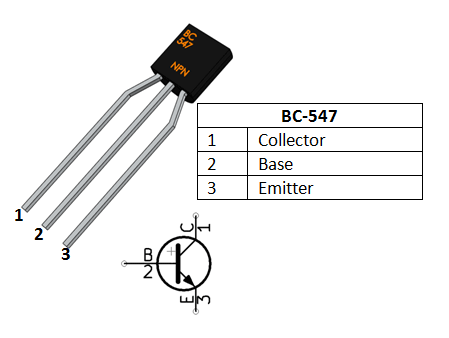
\includegraphics[scale=0.45]{figuras/fig1_BC547}
\centering
\end{figure}

	Basicamente, o coletor recebe uma tensão, o (terminal) base faz o chaveamento e emissor envia o sinal amplificado.

	O site Tecmundo\footnote{Disponível em \url{https://www.tecmundo.com.br/o-que-e/3596-o-que-e-um-transistor-e-porque-ele-e-importante-para-o-computador-.htm}} 
traz uma boa analogia sobre o funcionamento de um transitor como base onde ``(...)podemos pensar no transistor como uma torneira. O lado do cano que vem da rua é o terminal de entrada e o lado de onde sai a água 
é o terminal de saída. Quando você abre ou fecha a torneira, sua mão atua como o terminal do meio. Quanto mais você girar a 
torneira, mais água passará.''
	
\section{Corte e Saturação}

	O transistor pode trabalhar em 3 áreas de polarização: \textbf{ativa}, \textbf{corte} e \textbf{saturação}, conforme \autoref{figuras/fig2_GraficoArea}.
	Para esta experiência os pontos de corte e saturação são mais importantes. 
\begin{figure}[htb]
  \caption{\label{figuras/fig2_GraficoArea}Gráfico $I_c$ x $V_{ce}$ representando as áreas de polarização do transistor}
  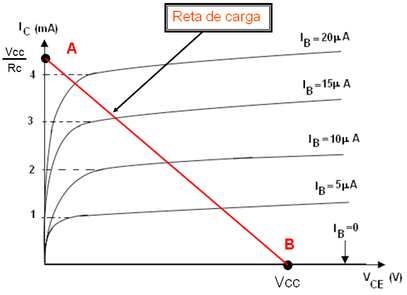
\includegraphics[scale=0.60]{figuras/fig2_GraficoArea}
  \centering
\end{figure}


A passagem da área de corte para a área de saturação é dada pela corrente aplicada na base ($I_b$). 

Quando $I_b = 0$, nosso transistor irá trabalhar na área de corte, o que significa que a corrente do coletor $I_c$ será nula. Desta forma temos: 
$$I_c = 0$$$$V_{ce} = V_{cc}$$

Já quando trabalhamos com $I_b >= I_{b_{sat}}$ o transistor operará na região de saturação onde $I_{c_{sat}} = \frac{V_{cc}}{R_c}$.
						



% ----------------------------------------------------------
% Descrever as etapas que devem ser realizadas para ... .
% contexto teórico abordado pelo assunto.
% ----------------------------------------------------------
% ----------------------------------------------------------
% Abordagem Teórica: Uma breve descrição que explique o 
% contexto teórico abordado pelo assunto.
% ----------------------------------------------------------

\chapter[Parte Prática]{Parte Prática}
%\addcontentsline{toc}{chapter}{Abordagem Teórica}
Em sala, montamos o circuito com base na esquemática da \autoref{figuras/fig3_CircuitoAula}.

\begin{figure}[htb]
  \caption{\label{figuras/fig3_CircuitoAula}Esquema de circuito com transistor como chave}
  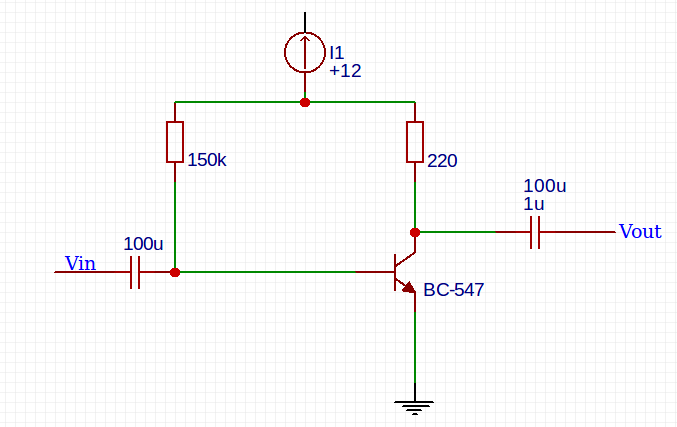
\includegraphics[scale=0.50]{figuras/fig3_CircuitoAula}
  \centering
\end{figure}

\section[Componentes e Equipamentos]{Componentes e Equipamentos} 

Abaixo os Componentes e equipamentos que foram utilizados nesta experiência:
\begin{itemize}
    \item 2x Capacitores de 100 $\mu$F
    \item 1x Resistor de 220 $\Omega$
    \item 1x Resistor de 150 k$\Omega$
    \item 1x Transistor BC547
    \item 1x Multímetro
    \item 1x Osciloscópio
    \item 1x Gerador de funções
    \item 1x Fonte de bancada
    \item 1x Protoboard
\end{itemize}


\section[Medições]{Medições}

\subsection{Tensões e Correntes}

As seguintes tensões foram medidas:

\par  $V_{CC}$= 12,00 V - $V_{RB}$= 11,44 V
\par  $V_{RC}$=  5,83 V - $V_{BE}$=  0,64 V 
\par  $V_{CE}$=  6,30 V - $V_{CE}$=  9,40 V 


Com esses valores aplicamos a lei de Ohm para calcular os valores das correntes, onde $V = R.I$:\\

$I_c=\frac{V_{RC}}{RC} = \frac{5,83}{220} = 26,5 mA$


$I_b=\frac{V_{RB}}{RB} = \frac{11,44}{150.10^3} = 0,076 mA$


$I_e= I_b + I_c = 26,576 mA$


\subsection[Gerador de Áudio]{Gerador de Áudio}

Para $f=1kHZ$, $V_{in}=0,1V_{pp}$, qual será o valor de $V_{out}$


Resposta:$0,1  V_{pp}$
\subsection{Valor máximo do sinal aplicado ao $V_{in}$}
Resposta: $8  V_{pp}$


% \section[Circuito]{Circuito}
% 
% Com os componentes citados no \autoref{Componentes e Equipamentos}, montamos o circuito abaixo:
% 
% \begin{figure}[htb]
%   \caption{\label{figuras/fig4_CircFinal}Circuito montado}
%   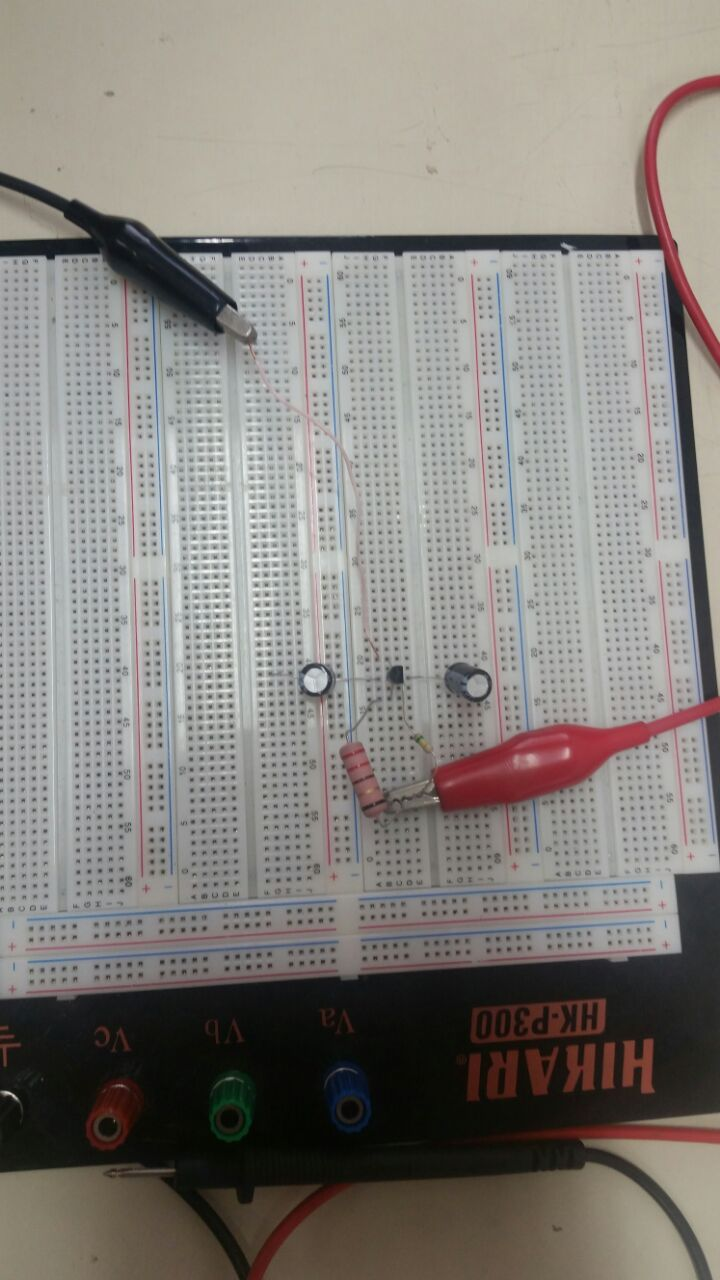
\includegraphics[scale=0.25]{figuras/fig4_CircFinal}
%   \centering
% \end{figure}
% ----------------------------------------------------------
% PARTE - preparação da pesquisa
% ----------------------------------------------------------
\nocite{transistoresIIUNESP}
\nocite{transistoresIFURJ}
\bibliography{refs}

\end{document}
